\documentclass{beamer}

\usepackage[numbering=fraction]{theme/beamerthemeCodeCourse}

\beamertemplatenavigationsymbolsempty

\title{yasd}
\subtitle{(yet another) self-driving car simulator}
\author{C. Caramaschi \and M. Biondi \and V. Armandi}
\institute{Alma Mater Studiorum $\cdot$ Università di Bologna\\
Corso di Laurea Magistrale in Informatica\\
Fisica dei Sistemi Complessi}
\date{December 2020}

\begin{document}

\maketitle

\begin{frame}
	\frametitle{yasd}
	\framesubtitle{(yet another) self-driving car simulator}

	\begin{center}
		\begin{block}{\textbf{What}}
			An isolated simulation environment designed to study how autonomous cars could learn to properly drive and coexist without an initial well defined traffic law
		\end{block}

		\begin{exampleblock}{\textbf{With}}
			\begin{itemize}
				\item a convoluted looped road track
				\item multiple autonomous cars
			\end{itemize}
		\end{exampleblock}

		\begin{alertblock}{\textbf{Without}}
			\setbeamercolor{itemize item}{fg=Marty}
			\begin{itemize}
				\item road signs
			\end{itemize}
		\end{alertblock}
	\end{center}
\end{frame}

\begin{frame}
	\frametitle{How}
	\framesubtitle{the system will work}

	The autonomous cars should learn to:
	\begin{center}
		\begin{exampleblock}{\textbf{Respect}}
			\begin{itemize}
				\item safety distance
				\item speed limits
				\item precedence
			\end{itemize}
		\end{exampleblock}

		\begin{alertblock}{\textbf{Avoid}}
			\setbeamercolor{itemize item}{fg=Marty}
			\begin{itemize}
				\item border collisions
				\item road accidents
				\item traffic congestion
			\end{itemize}
		\end{alertblock}
	\end{center}
\end{frame}

\begin{frame}
	\frametitle{Why}
	\framesubtitle{are we developing it?}

	\begin{block}{}
		\setbeamercolor{itemize item}{fg=TealDrop}
		To study how self-driving cars could learn to coexist autonomously following traffic rules not previously defined
		\setbeamercolor{itemize item}{fg=TealDrop}
		\begin{itemize}
			\item To which side should priority be given to at a crossroad?
			\item On which side should an overtaking manoeuvre carried out?
		\end{itemize}
	\end{block}
\end{frame}

\begin{frame}
	\frametitle{Neural Network}


	\begin{figure}[ht]
		\centering
		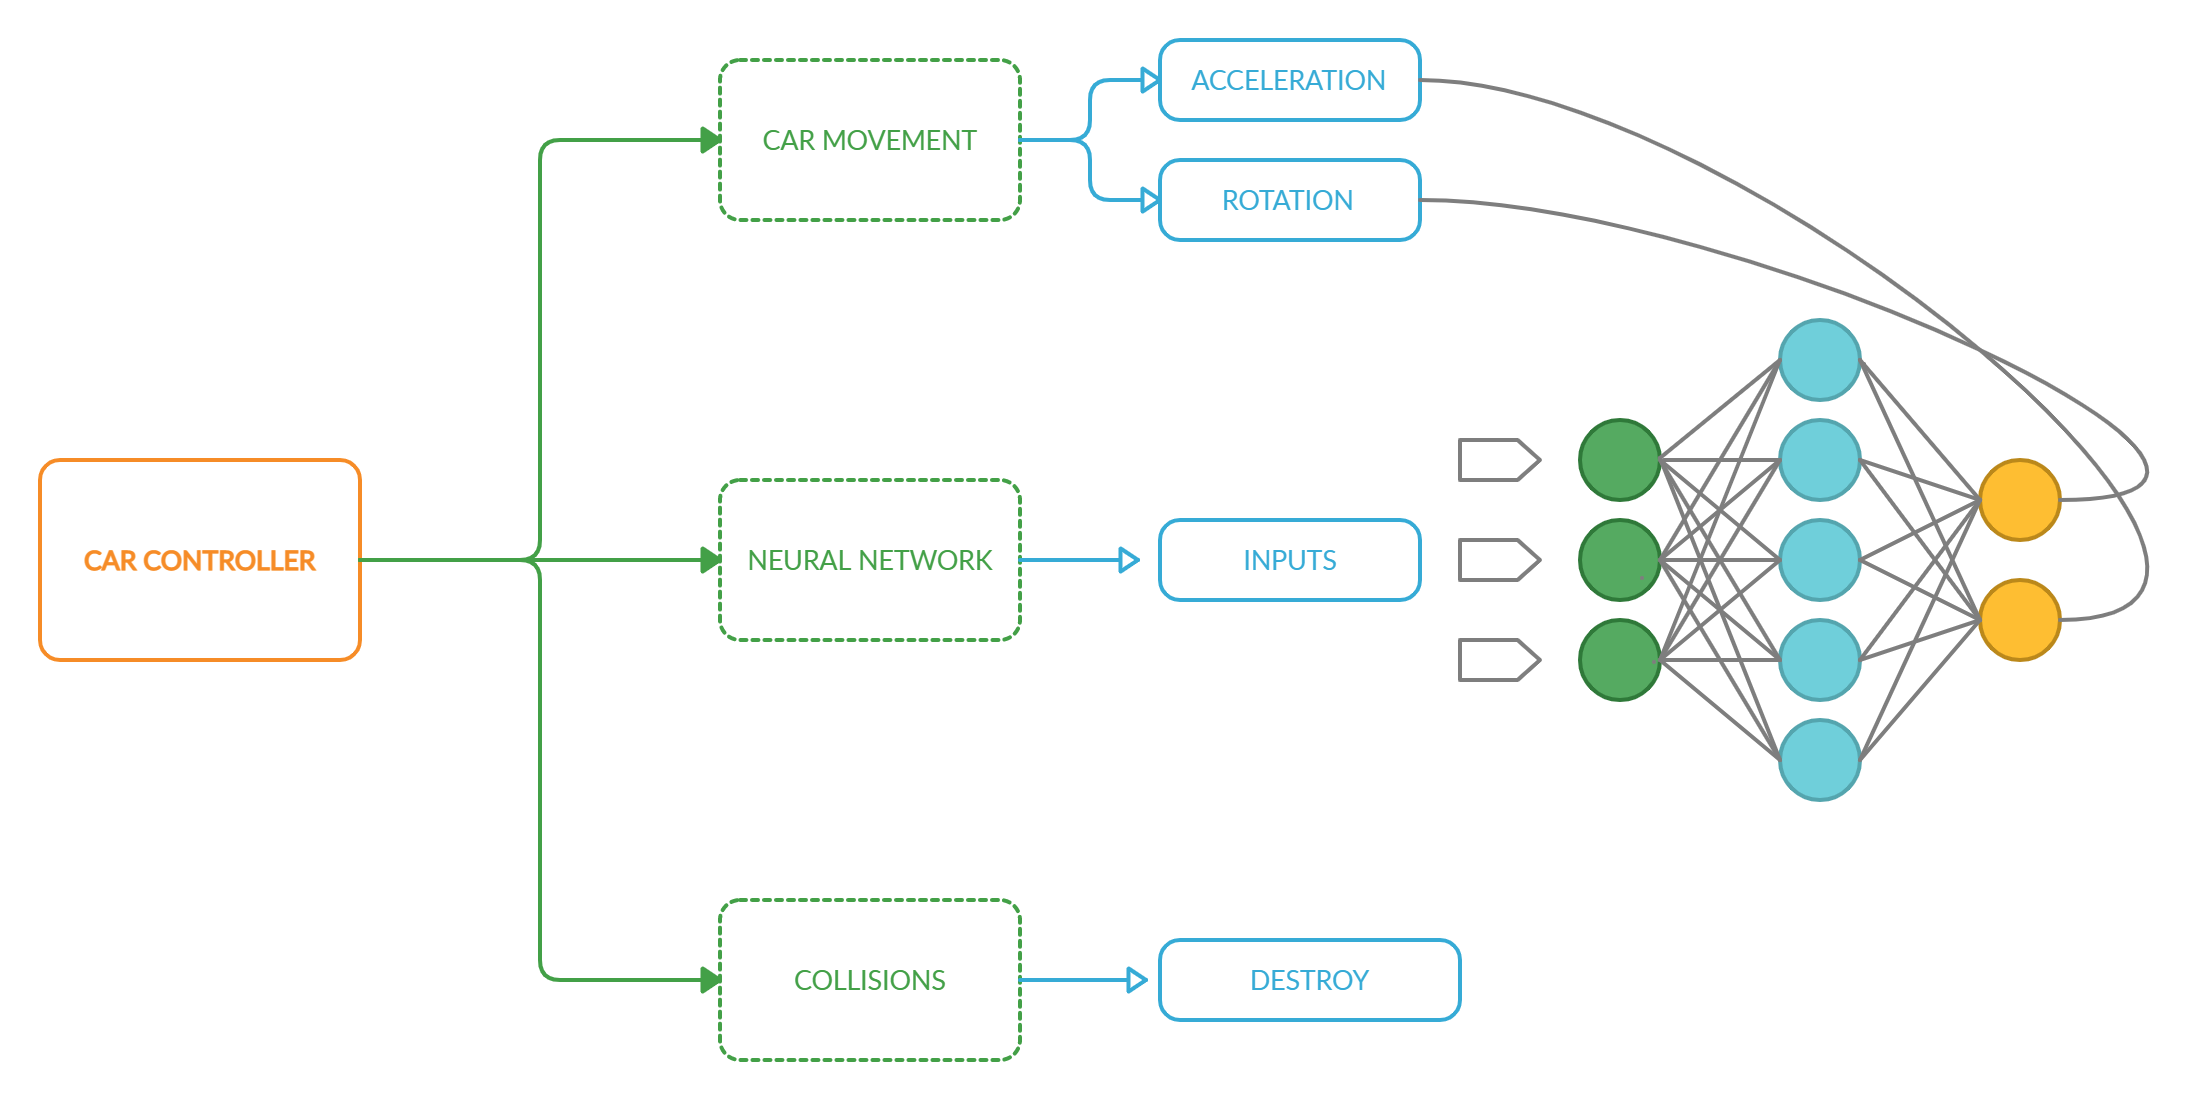
\includegraphics[width=10cm]{images/neural_network_scheme.png}
	\end{figure}

\end{frame}

\begin{frame}
	\frametitle{Genetic Algorithm}

	\begin{figure}[ht]
		\centering
		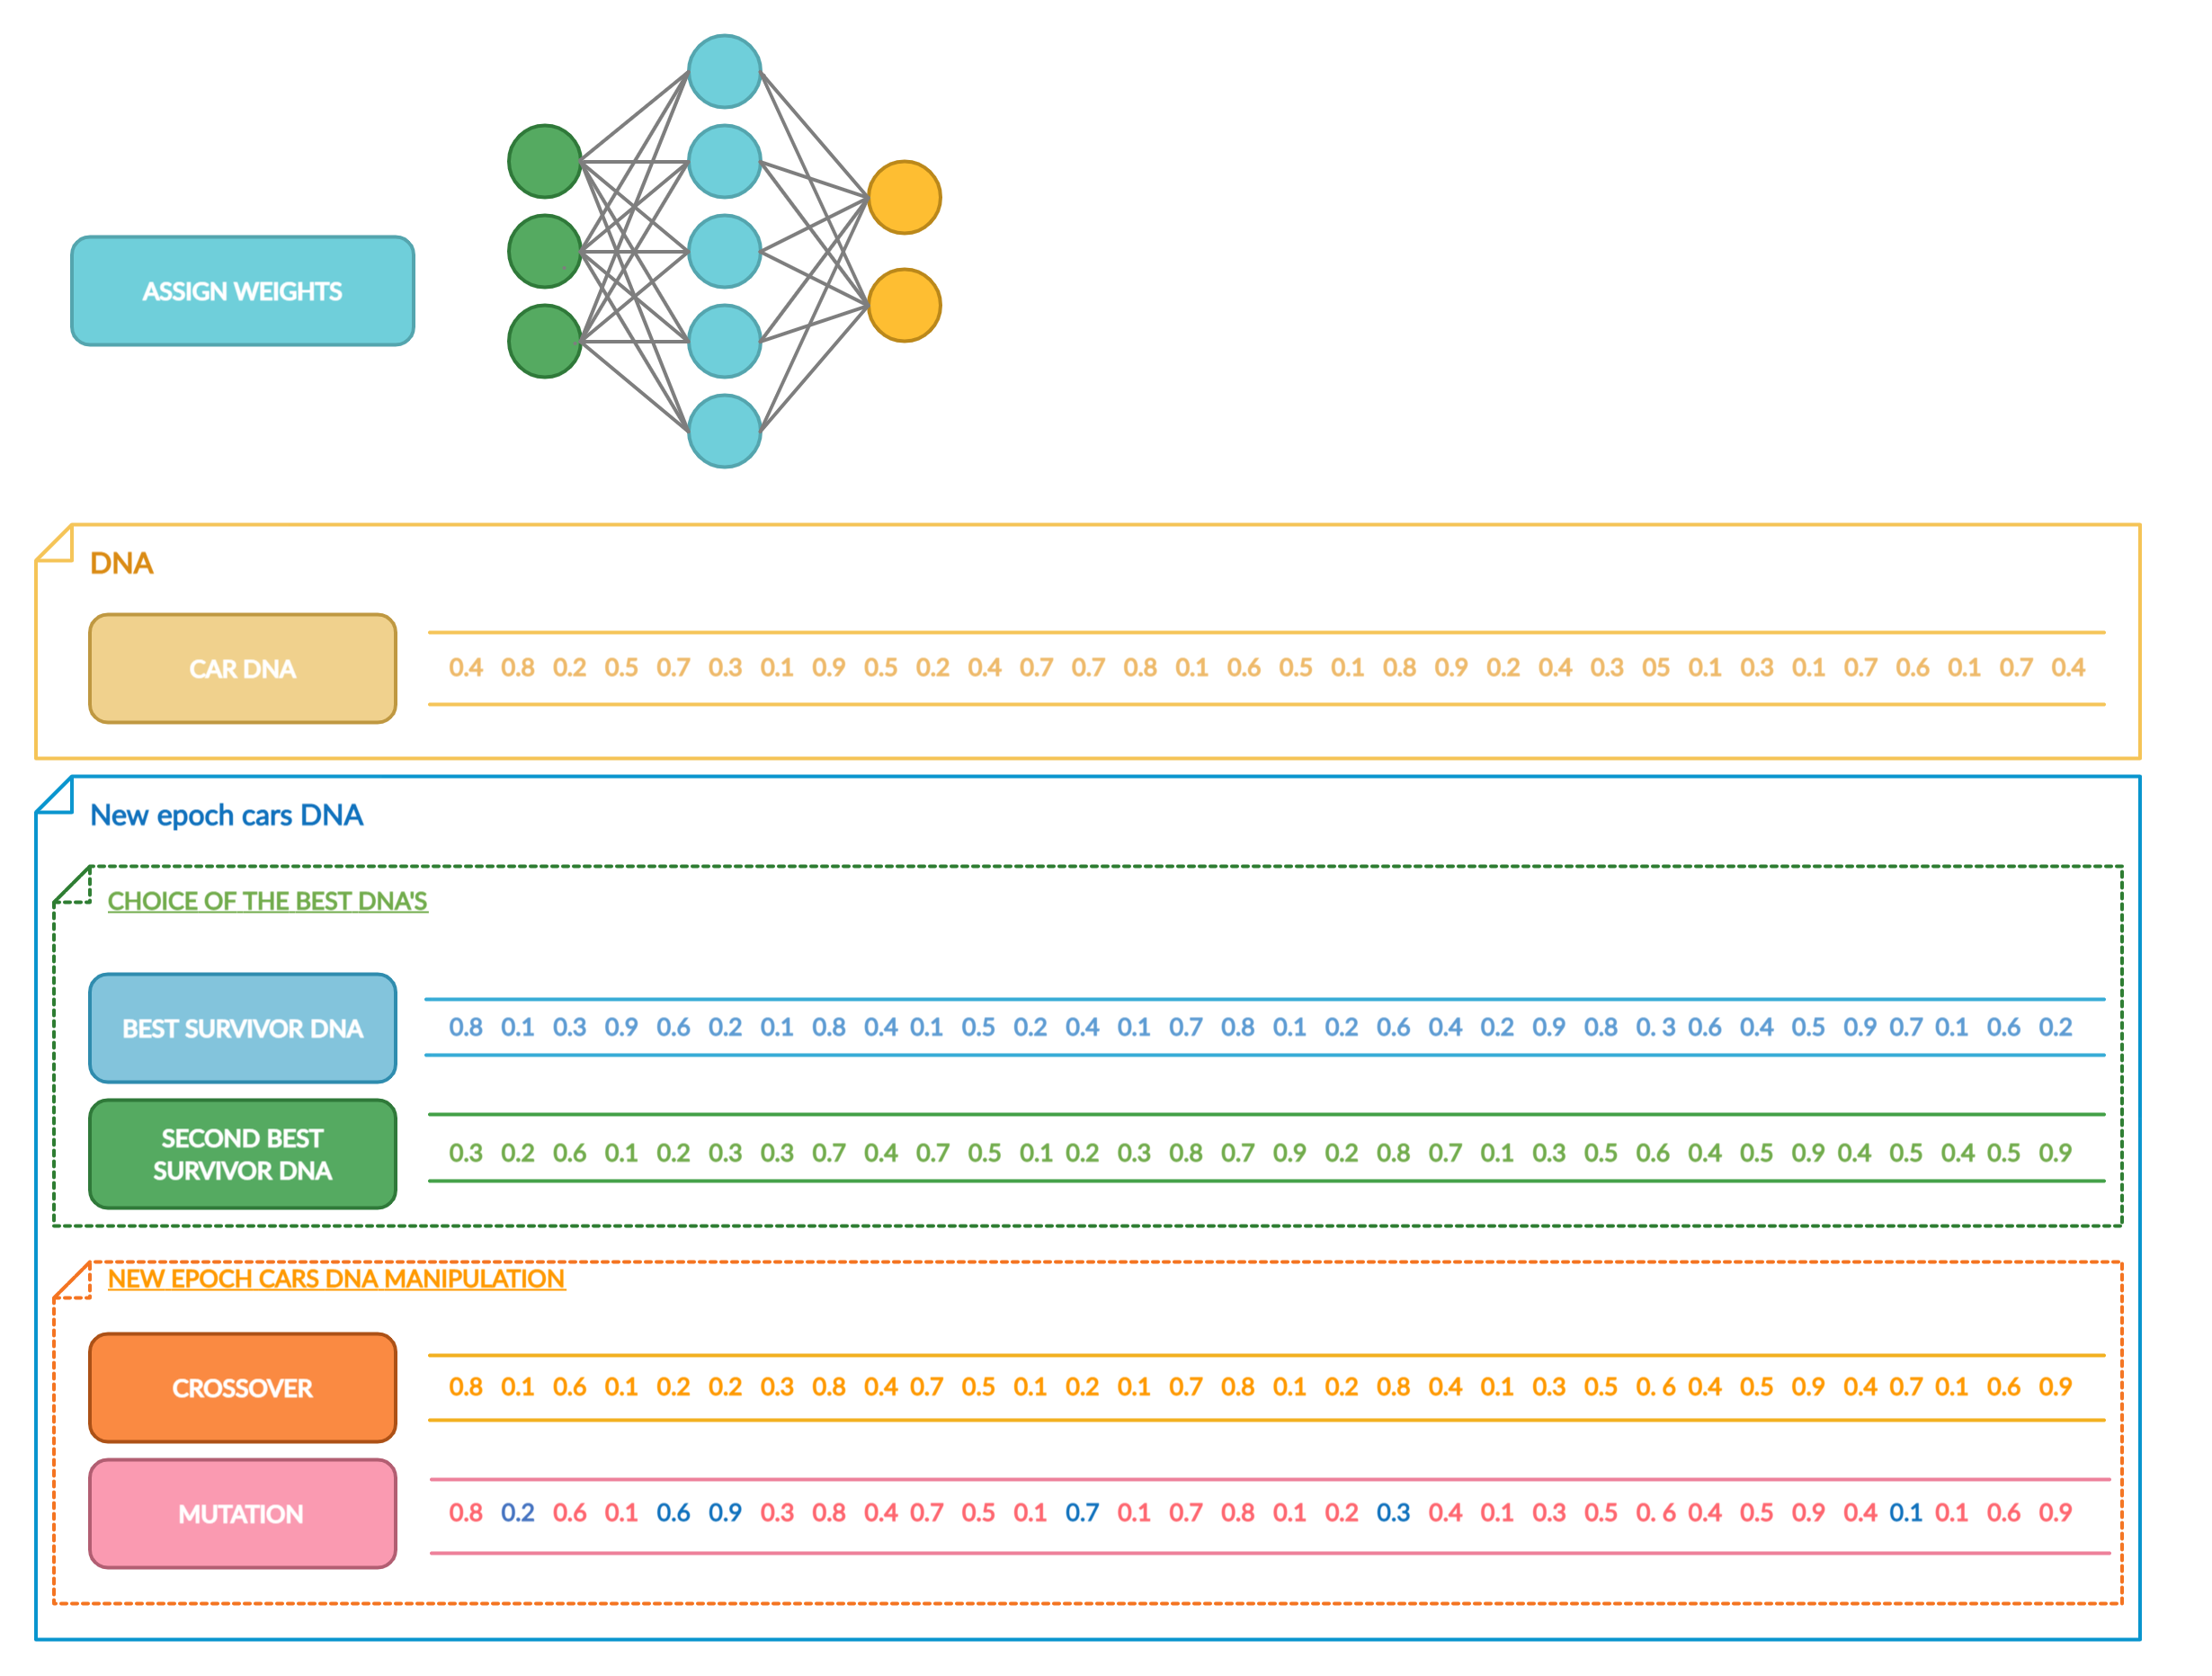
\includegraphics[width=10cm]{images/genetic_algorithm.png}
	\end{figure}

\end{frame}

\begin{frame}
	\frametitle{Neural Network \& Genetic Algorithm}

	\begin{figure}
		\centering
		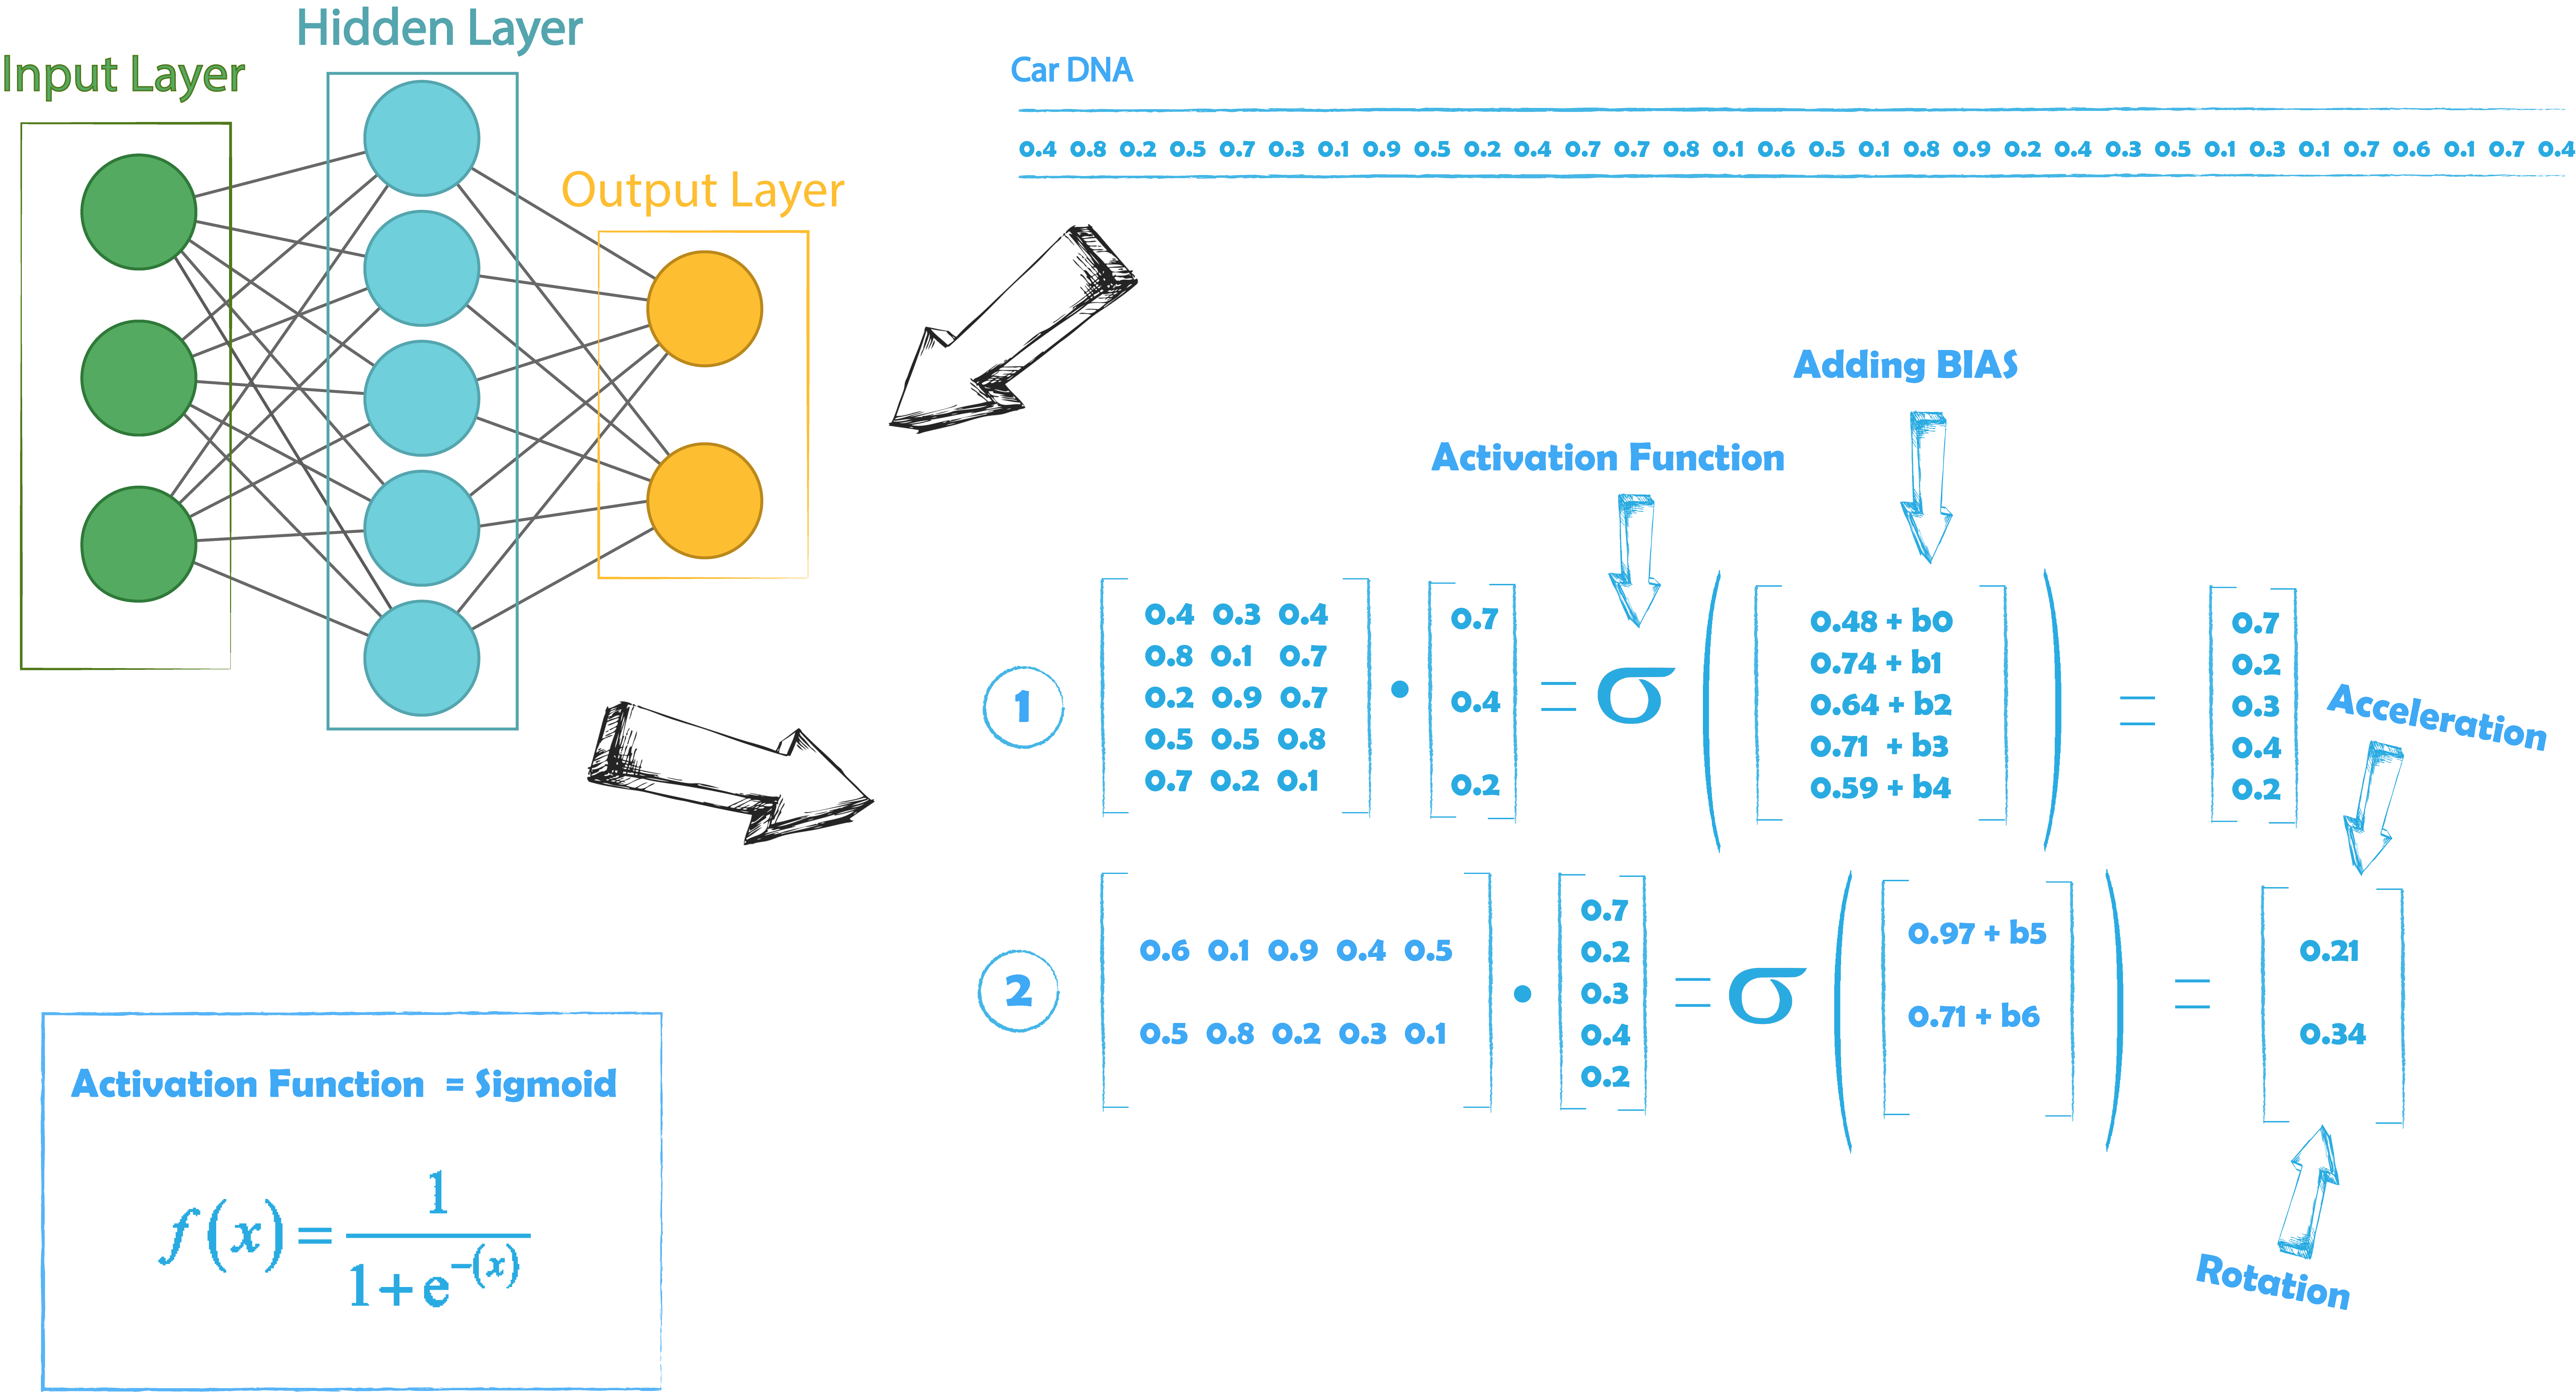
\includegraphics[width=11cm]{images/NN.png}
	\end{figure}

\end{frame}

\begin{frame}
	\frametitle{Track}
	\framesubtitle{generation process}

	\begin{exampleblock}{}
		\begin{enumerate}
			\item input track parameters
			      \begin{itemize}
				      \item number of crossroads
				      \item speed limit
				      \item coefficient of friction
			      \end{itemize}
			\item Lissajous curve algorithm
			\item track drawing using graphic libraries
		\end{enumerate}
	\end{exampleblock}

	\begin{figure}
		\centering
		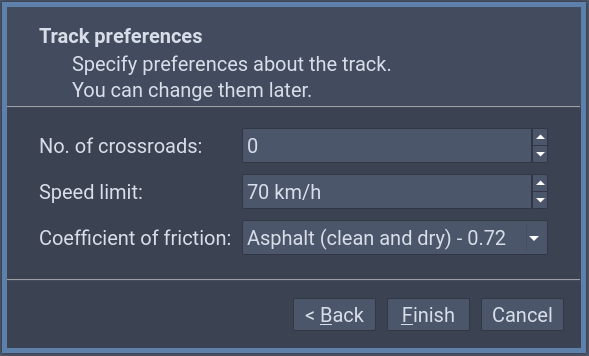
\includegraphics[scale=0.25]{images/yasd-track.png}
	\end{figure}
\end{frame}

\begin{frame}
	\frametitle{Lissajous}
	\framesubtitle{curve algorithm}

	\begin{block}{\textbf{Use}}
		\setbeamercolor{itemize item}{fg=TealDrop}
		\begin{itemize}
			\item simple curves
			\item good positioning of crossroads
		\end{itemize}
	\end{block}

	\begin{exampleblock}{\textbf{Formulas}}
		\begin{itemize}
			\item  \[x=A_{x}\sin(\omega _{x}t+\phi _{x})\]
			\item  \[y=A_{y}\sin(\omega _{y}t+\phi _{y})\]
		\end{itemize}
	\end{exampleblock}
\end{frame}

\begin{frame}
	\frametitle{Car}
	\framesubtitle{types}

	\begin{alertblock}{\textbf{Red car}}
		\setbeamercolor{itemize item}{fg=Marty}
		\begin{itemize}
			\item driving speed $\approx$ speed limit
			\item low proximity sensors sensitivity
		\end{itemize}
	\end{alertblock}

	\begin{exampleblock}{\textbf{Green car}}
		\begin{itemize}
			\item driving speed $\le$ speed limit
			\item normal proximity sensors sensitivity
		\end{itemize}
	\end{exampleblock}

	\begin{block}{\textbf{Blue car}}
		\setbeamercolor{itemize item}{fg=TealDrop}
		\begin{itemize}
			\item driving speed $\ll$ speed limit
			\item high proximity sensors sensitivity
		\end{itemize}
	\end{block}

\end{frame}

\begin{frame}
	\frametitle{Editing preferences}
	\framesubtitle{from the second epoch onwards}

	\begin{exampleblock}{\textbf{Yes - Track preferences}}
		\begin{itemize}
			\item number of crossroads
			\item speed limit
			\item coefficient of friction
		\end{itemize}
	\end{exampleblock}

	\begin{alertblock}{\textbf{No - Set of cars}}
		\setbeamercolor{itemize item}{fg=Marty}
		\begin{itemize}
			\item number of red cars
			\item number of green cars
			\item number of blue cars
		\end{itemize}
	\end{alertblock}
\end{frame}

\begin{frame}
	\frametitle{.yasd}
	\framesubtitle{file extension}
	{\tt
	~~~~~~~~\{\\
	~~~~~~~~~~~~"cars": [\{\\
	~~~~~~~~~~~~~~~~"id": 0,\\
	~~~~~~~~~~~~~~~~"color": "red",\\
	~~~~~~~~~~~~~~~~"dna": [0.1,0.6,...,0.7]\\
	~~~~~~~~~~~~\}],\\
	~~~~~~~~~~~~"track": \{\\
	~~~~~~~~~~~~~~~~"crossroads": 7,\\
	~~~~~~~~~~~~~~~~"friction": 0,\\
	~~~~~~~~~~~~~~~~"limit": 70\\
	~~~~~~~~~~~~\}\\
	~~~~~~~~\}\\
	}
\end{frame}

\begin{frame}
	\frametitle{Technical details}
	\framesubtitle{about the project}

	\begin{block}{\textbf{Programming language}}
		\setbeamercolor{itemize item}{fg=TealDrop}
		\begin{itemize}
			\item C++
		\end{itemize}
	\end{block}
	\begin{exampleblock}{\textbf{GUI}}
		\begin{itemize}
			\item Qt5 + OpenGL
		\end{itemize}
	\end{exampleblock}
	\begin{block}{\textbf{Building process}}
		\setbeamercolor{itemize item}{fg=TealDrop}
		\begin{itemize}
			\item CMake
		\end{itemize}
	\end{block}
	\begin{exampleblock}{\textbf{Source Code}}
		\begin{itemize}
			\item GitHub
			\item GPL-3.0
		\end{itemize}
	\end{exampleblock}
\end{frame}

\begin{frame}
	\frametitle{Future developments}
	\framesubtitle{ }

	\begin{block}{}
		\setbeamercolor{itemize item}{fg=TealDrop}
		\begin{itemize}
			\setbeamercolor{itemize item}{fg=TealDrop}
			\item Reinforcement learning (RL)
			\item Pictures as sensors input
		\end{itemize}
	\end{block}
\end{frame}
\end{document}
